Aside from the applied density fitting method also the osed orbital free basis set has an aguably even larger effect on the accuracy of the density fitted density.
The often used even tempered besis set are an reliable, when also inefficient way to define an orbital free bassis set. Their simple construction algorith\cite{cosnt} covers the space of possible densities very broadly without.
To improve the performance of our orbital free basis set it makes sense to use ab basis set which offers a higher  resolution in regions where densities fluctuate more rapitly.
We construct this improved basis by starting with an even tempered one and used differentiable integrals and autograd to .

\section{Using differentiable integrals to optimize an orbital free basis set}
The basis density fitting formulation which minimizes the L2 norm of the residual density is given by:
The following Lagragien describes the residula density
\begin{align}
    \mathcal{L}[\rho] &= \min_{\rho'}\left(||\rho-\rho'||_{\text{L2}}\right)\\
    & = \min_{\{p_{\mu}\}_{\mu \in 1,...,n_b}} p^\mu W_{\mu,\nu} p^\nu - 2 p^\mu L^{\mu,\gamma\sigma} \Gamma^{\gamma\sigma} + \Gamma^{\mu\nu} D_{\mu\nu,\gamma\sigma} \Gamma^{\gamma,\sigma}
    & = \left[p^\mu W_{\mu,\nu} p^\nu - 2 p^\mu L^{\mu,\gamma\sigma} \Gamma^{\gamma\sigma}\right]_{\mathbf{p} = W^{-1}\bar{L}\bar\Gamma}
    & = \bar \Gamma \bar L ^T W^{-1} \bar L \bar Gamma - 2 \bar Gamma \bar L^T W^{-1} \bar L \bar \Gamma + \bar \Gamma \bar D \bar Gamma
    & = - \bar Gamma \bar L^T W^{-1} \bar L \bar \Gamma + \bar \Gamma \bar D \bar Gamma
\end{align}
We can now insert the dependency of our integrals on the exponents $\{\mathbf{\alpha}_Z\}_{Z\in \text{H,C,N,O,F}}$ for the gaussian basis functions for each atom.
The dependent integrals are the two center integral $W_{\mu,nu}(\mathbf{\alpha}) = \langle \omega_\mu(\mathbf{\alpha})|\omega_\nu(\mathbf{\alpha})\rangle$
 and the three center overlap integral $L_{\mu,\gamma\sigma}(\mathbf{\alpha}) = \langle \omega_\mu(\mathbf{\alpha})|\eta_\gamma\eta_\sigma\rangle$. The 4 center overlap integral does not depend on the orbital free basis functions $\omega_\mu(\mathbf{\alpha})$ and can therefor be omitted from the final loss when doing gradient decent.
 \begin{align}\label{loss_basis_set_fitting}
    \text{Loss}(\mathbf{\alpha}) & = - \bar \Gamma \bar L^T(\mathbf{\alpha}) W^{-1}(\mathbf{\alpha}) \bar L(\mathbf{\alpha}) \bar \Gamma
 \end{align}
 Other formulations using the residual hartree energy can also be easily formulated but they are much more computational expensive and therefor not as usefull for this procedere.
 \subsection{Comparison of performance of fitted bsis sets with vanilla even tempered basis sets}
 We compare several fitted basis sets originating from even tempered basis sets with $\beta$ equal to 5 3 or 2.5 on the same metrics that we used for the different density fitting methods. For better readability we only compare them first using the density fitting method hartree+external Mofdft as it.
 \section{Additional Sidelosses}
 Using the prior mentioned loss\ref{loss_basis_set_fitting} alone isn't sufficient to garantie that the fitted basis set produces stable labels As can be seen the in the following plots, the exponents of basis set ... have moved very close together and lead to quite unstable coefficients. While the metrics of this basis set are very good, it has considerable problems while training. \ref{plot_tensorboard}.
 To counteract this behavior additional sidelosses on the fitted coefficients $\mathbf{p}(\mathbf{alpha}) = W^{-1}(\mathbf{\alpha}) \bar L(\mathbf{\alpha}) \bar \Gamma$ during training have been applied. 
 \begin{align}
    \text{Loss}_\text{Coeffs}(\mathbf{\alpha}) = \epsilon_\text{Coeffs}||*\mathbf{p}(\mathbf{alpha})||^2\\
    \text{Loss}_\text{STD\_Coeffs}(\mathbf{\alpha}) = \epsilon_\text{STDCoeffs}\left(\text{std}(\mathbf{p}(\mathbf{alpha}))\right)^2\\
    \text{Loss}_\text{STD\_Coeffs\_Diff}(\mathbf{\alpha}) = \epsilon_\text{STDCoeffs}\left(\text{std}(\mathbf{p}(\mathbf{alpha}))\right)^2\\
 \end{align}

 Where the standart deviation is computed using A running STD implementation following welfords algorithm \cite{Welford}. 
 The following plots show how the metrics change after aplliing these additional sidelosses starting with the previously best performing basis sets.
 After applying these algorithms the standart deviation of the is much more evenly distributed over the coefficients. 
 Which also results in smoother training.

 At last we are going to compare the performance of a typical transformer model trained on the different fitted basis sets when doing denop and find out that while they aren't better at fitting the produced labels, they still perform better when compared to the orbital free density and lower the theoretical best performance.

\begin{figure}
    \centering
    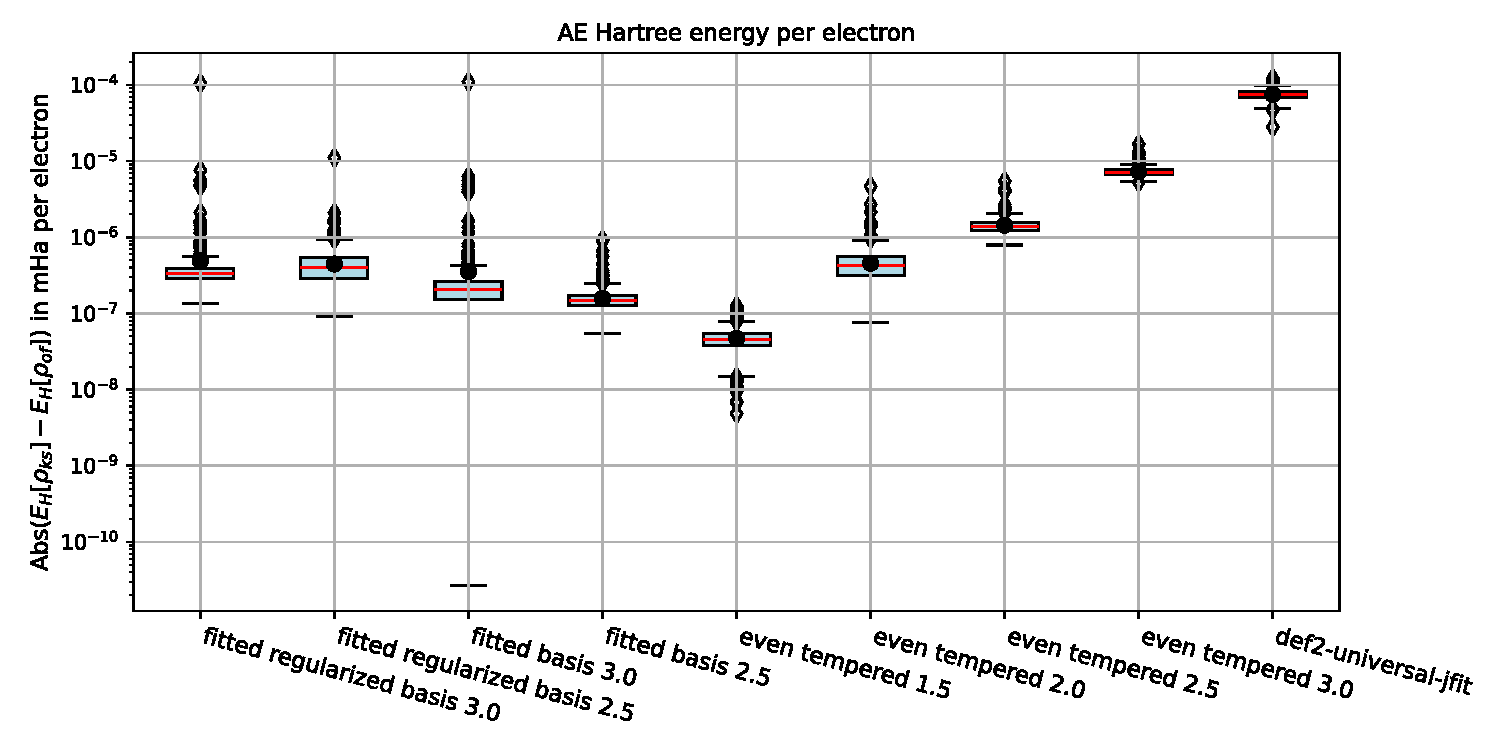
\includegraphics[width=0.6\textwidth]{chapters/results/results_images/AE_hartree_energy_on_hartree+external_MOFDFT_for_different_basis_sets}
    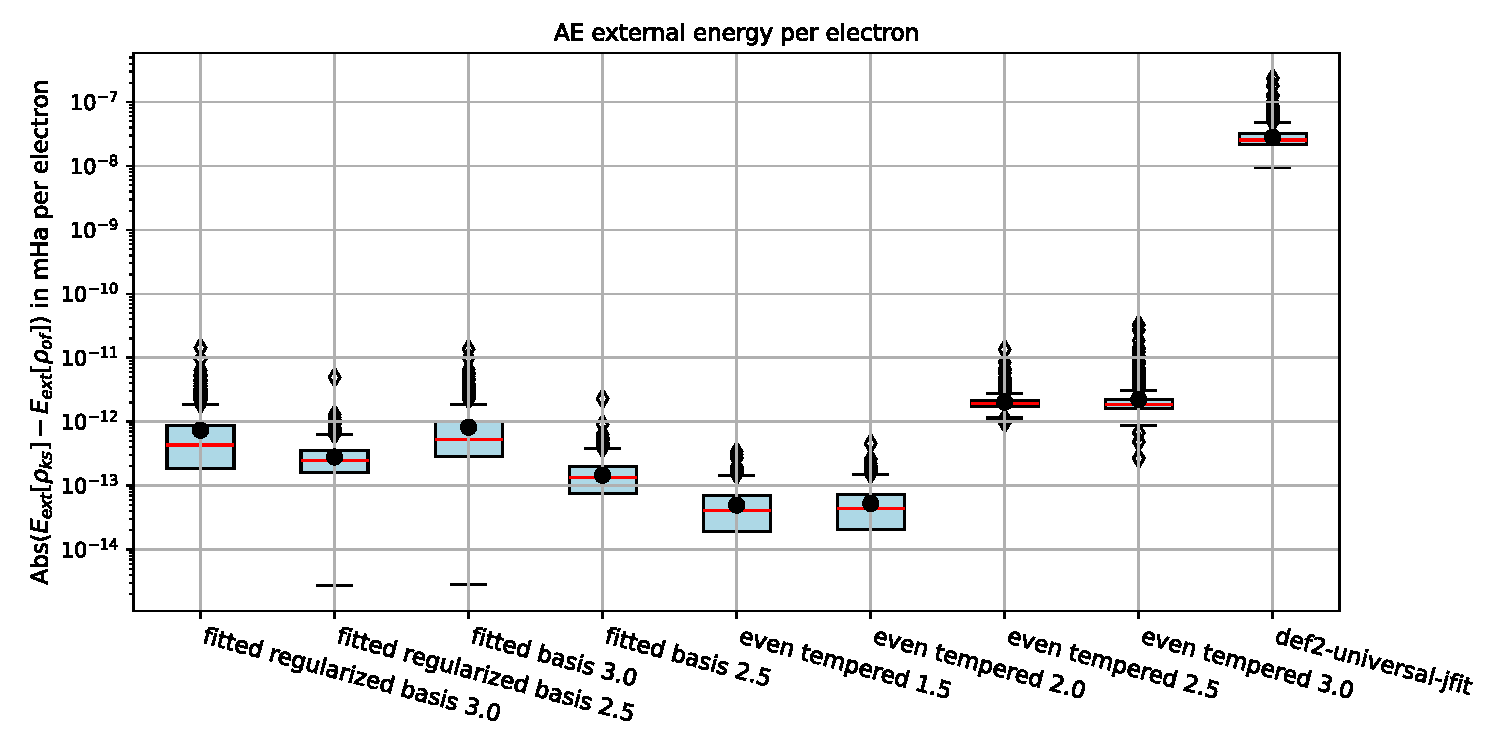
\includegraphics[width=0.6\textwidth]{chapters/results/results_images/AE_ext_energy_on_hartree+external_MOFDFT_for_different_basis_sets}
    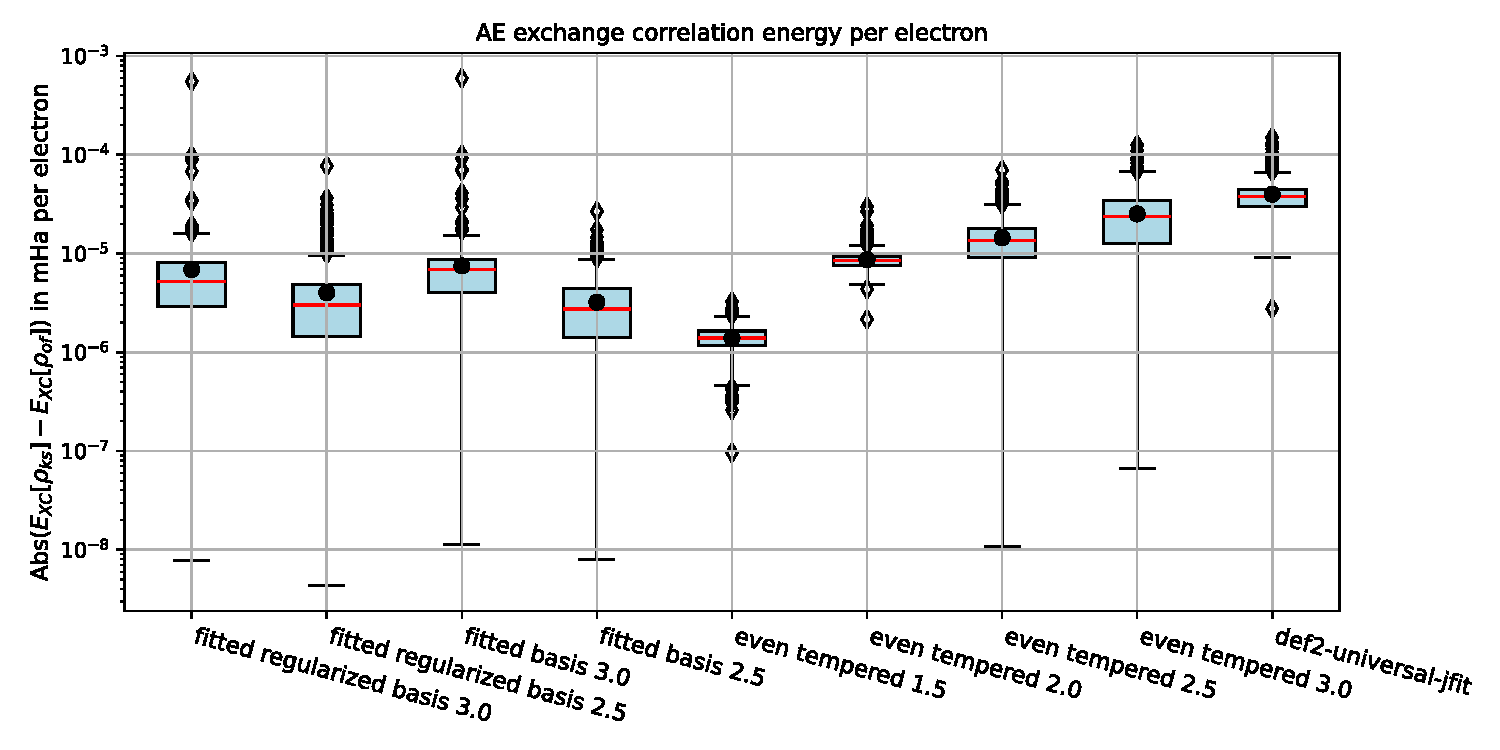
\includegraphics[width=0.6\textwidth]{chapters/results/results_images/AE_xc_energy_on_hartree+external_MOFDFT_for_different_basis_sets}
    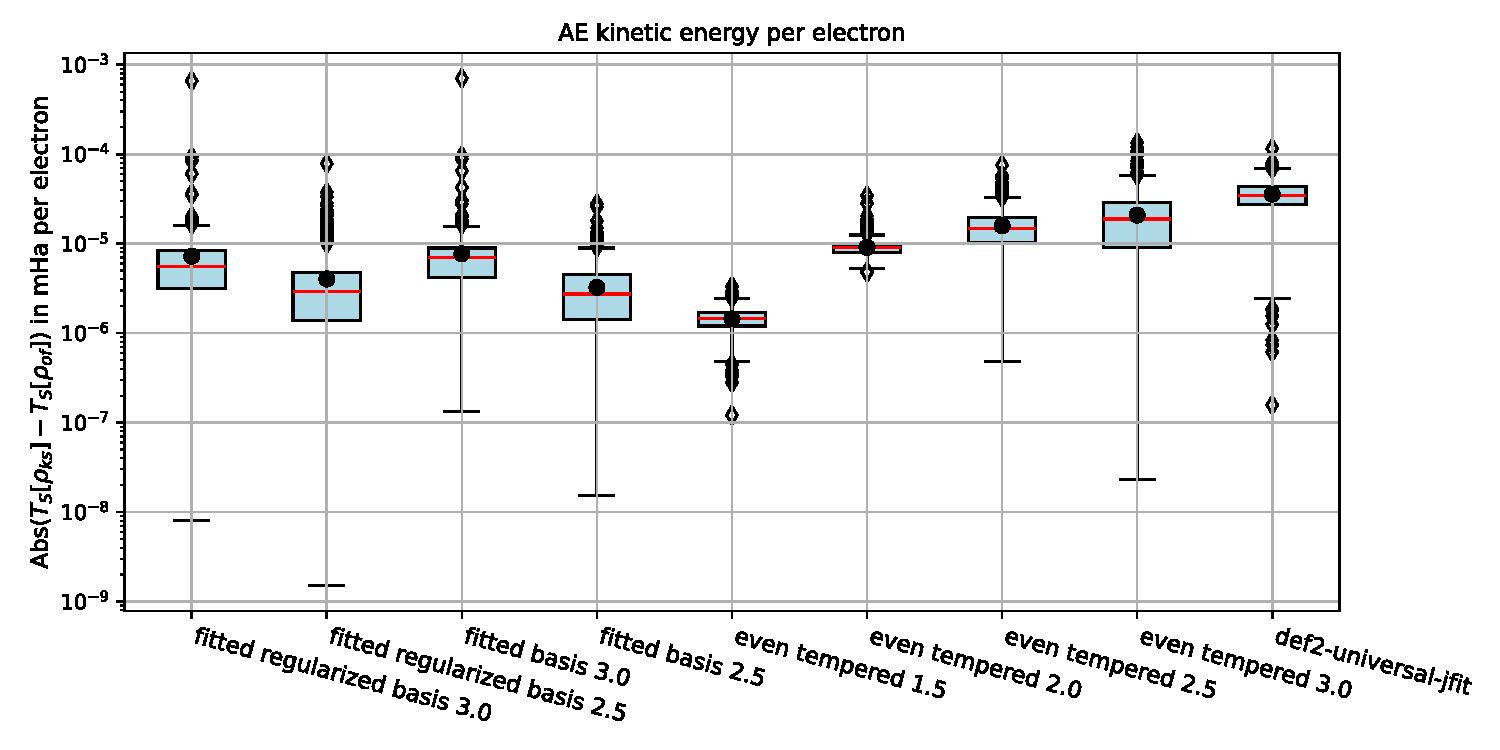
\includegraphics[width=0.6\textwidth]{chapters/results/results_images/AE_kin_energy_on_hartree+external_MOFDFT_for_different_basis_sets}
    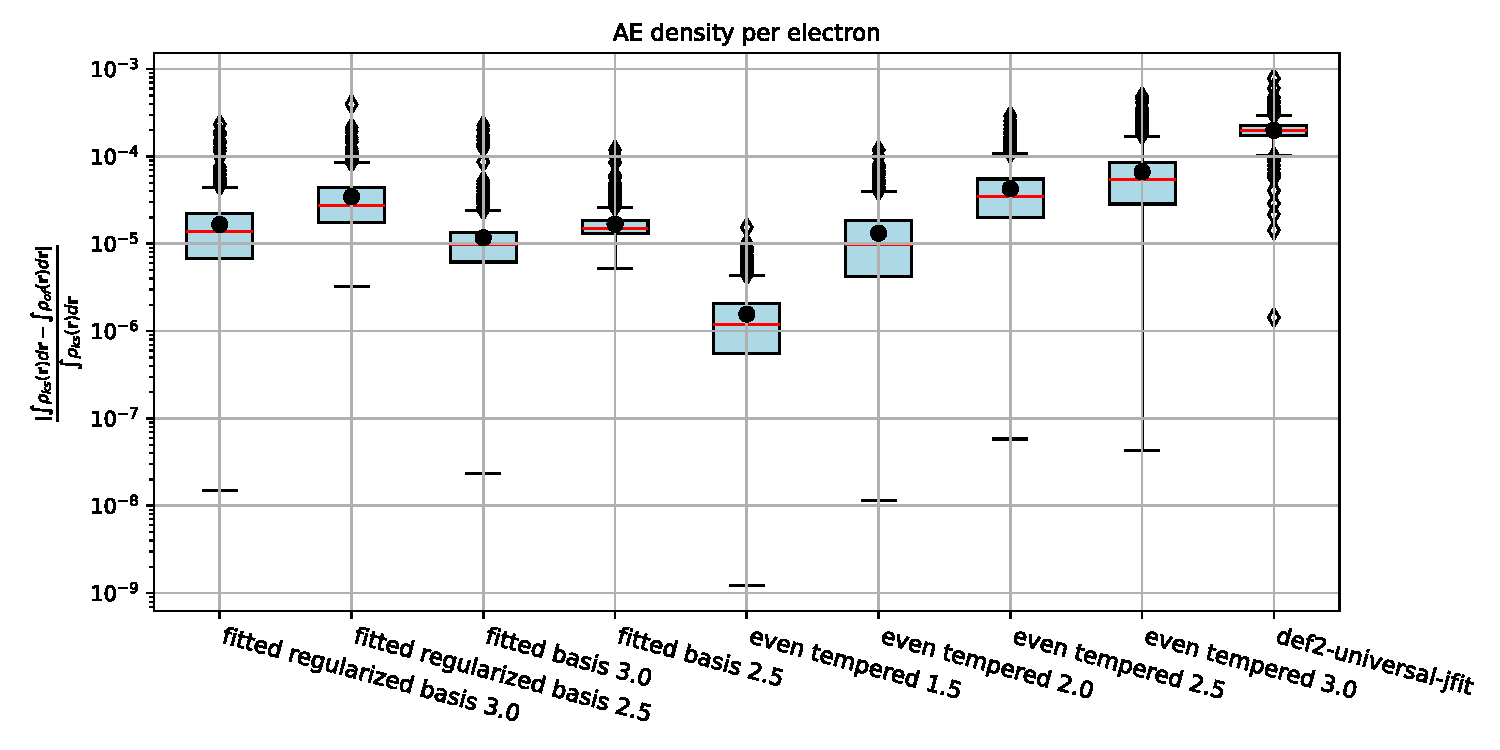
\includegraphics[width=0.6\textwidth]{chapters/results/results_images/AE_density_on_hartree+external_MOFDFT_for_different_basis_sets}
    \caption{Comparison of the different losses used to fit the basis set}
\end{figure}
\begin{figure}
    \centering
    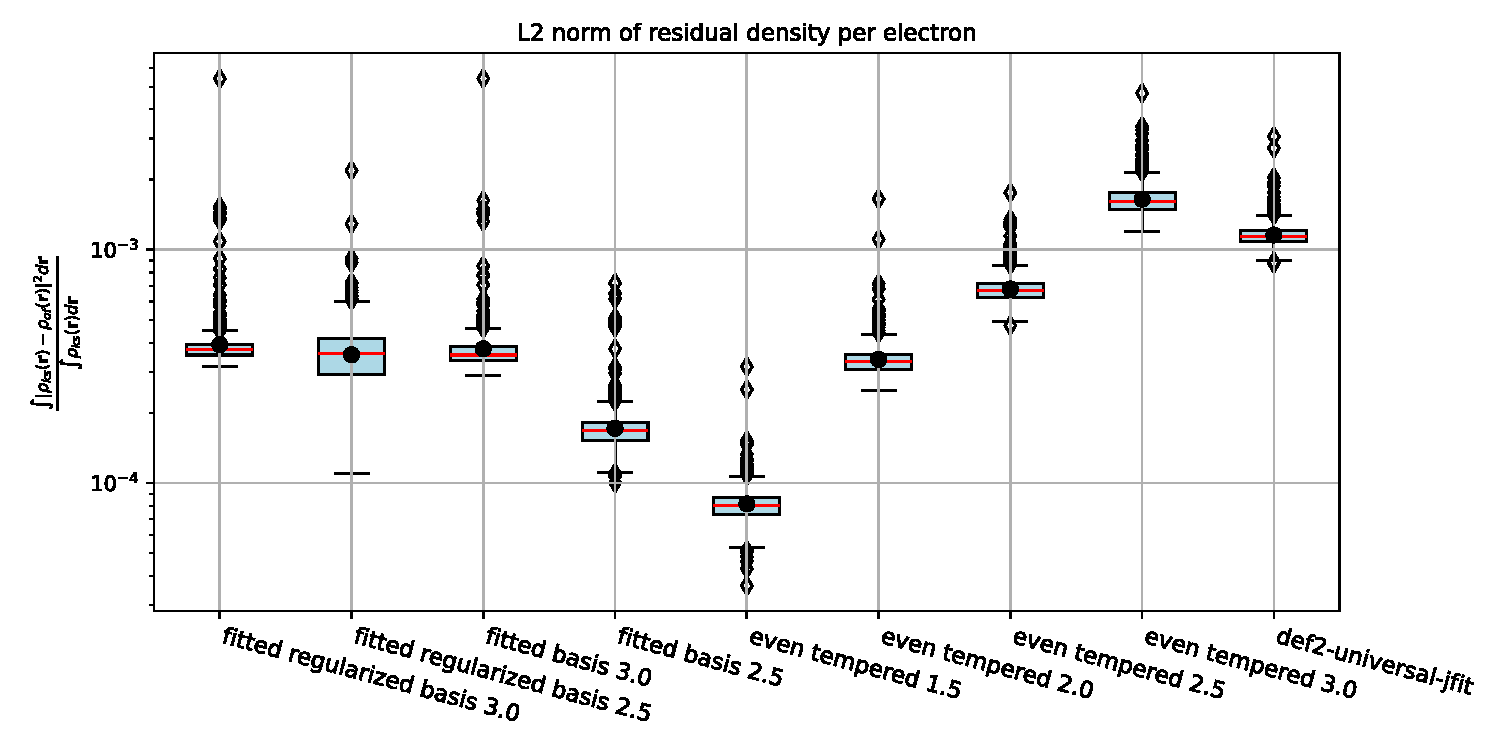
\includegraphics[width=0.6\textwidth]{chapters/results/results_images/L2_residual_densities_on_hartree+external_MOFDFT_for_different_basis_sets}
    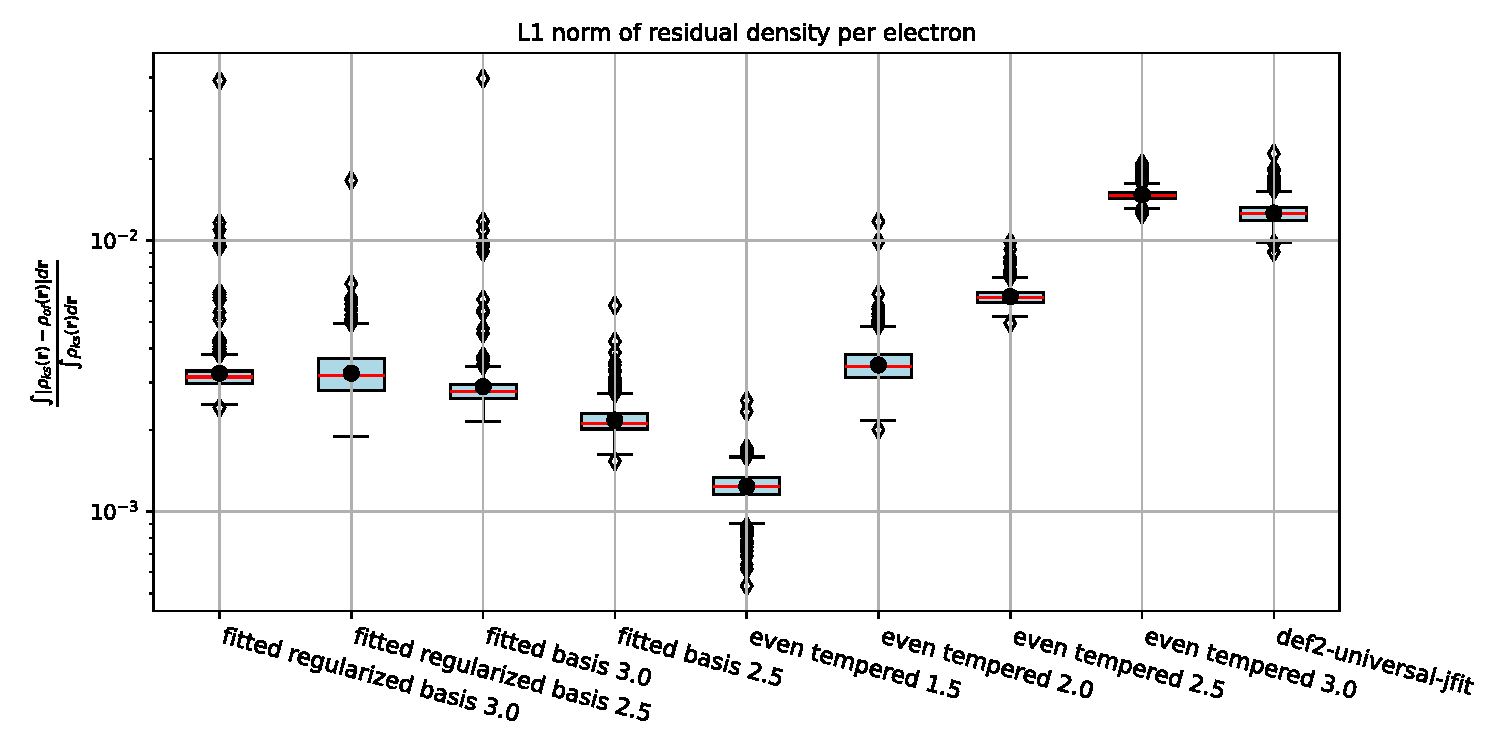
\includegraphics[width=0.6\textwidth]{chapters/results/results_images/L1_residual_densities_on_hartree+external_MOFDFT_for_different_basis_sets}
    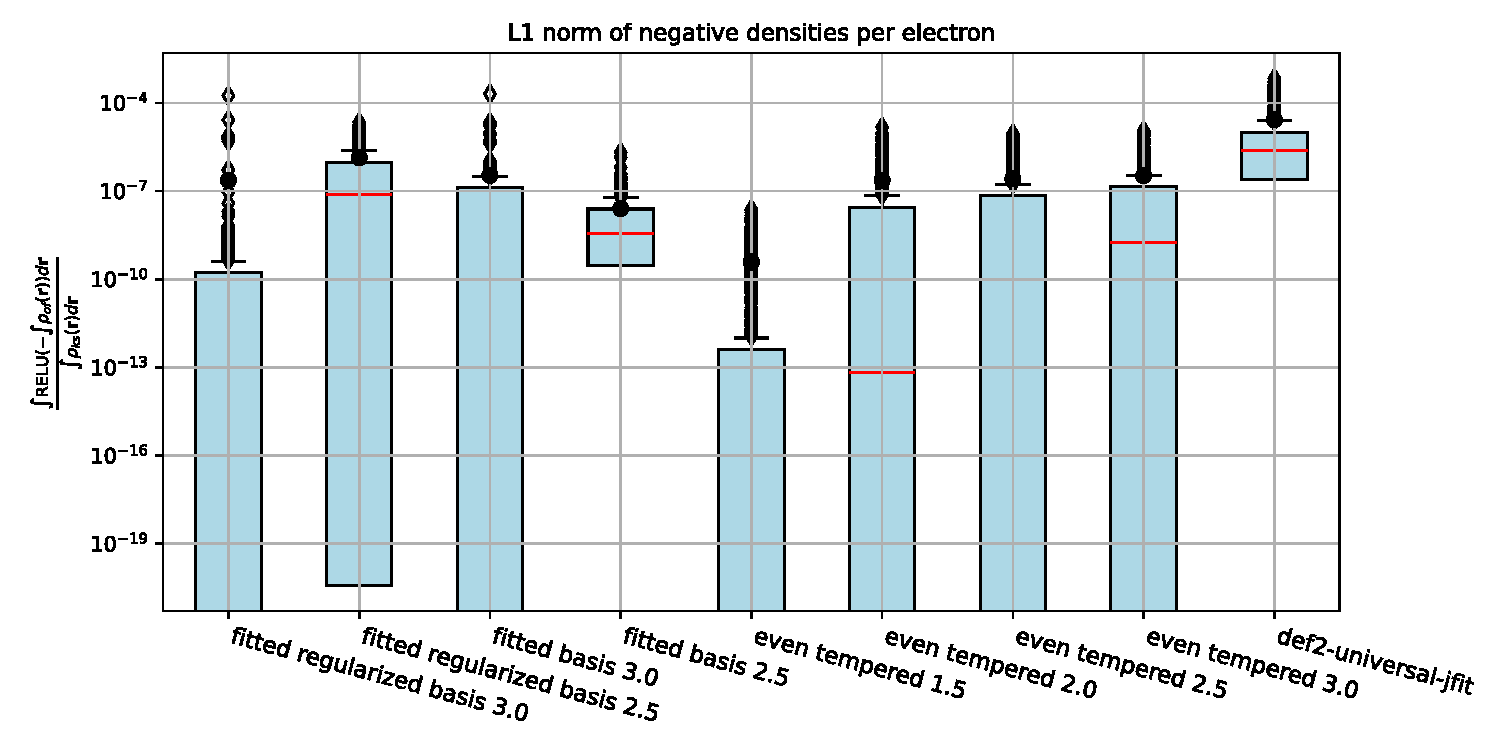
\includegraphics[width=0.6\textwidth]{chapters/results/results_images/L1_negative_densities_on_hartree+external_MOFDFT_for_different_basis_sets}
    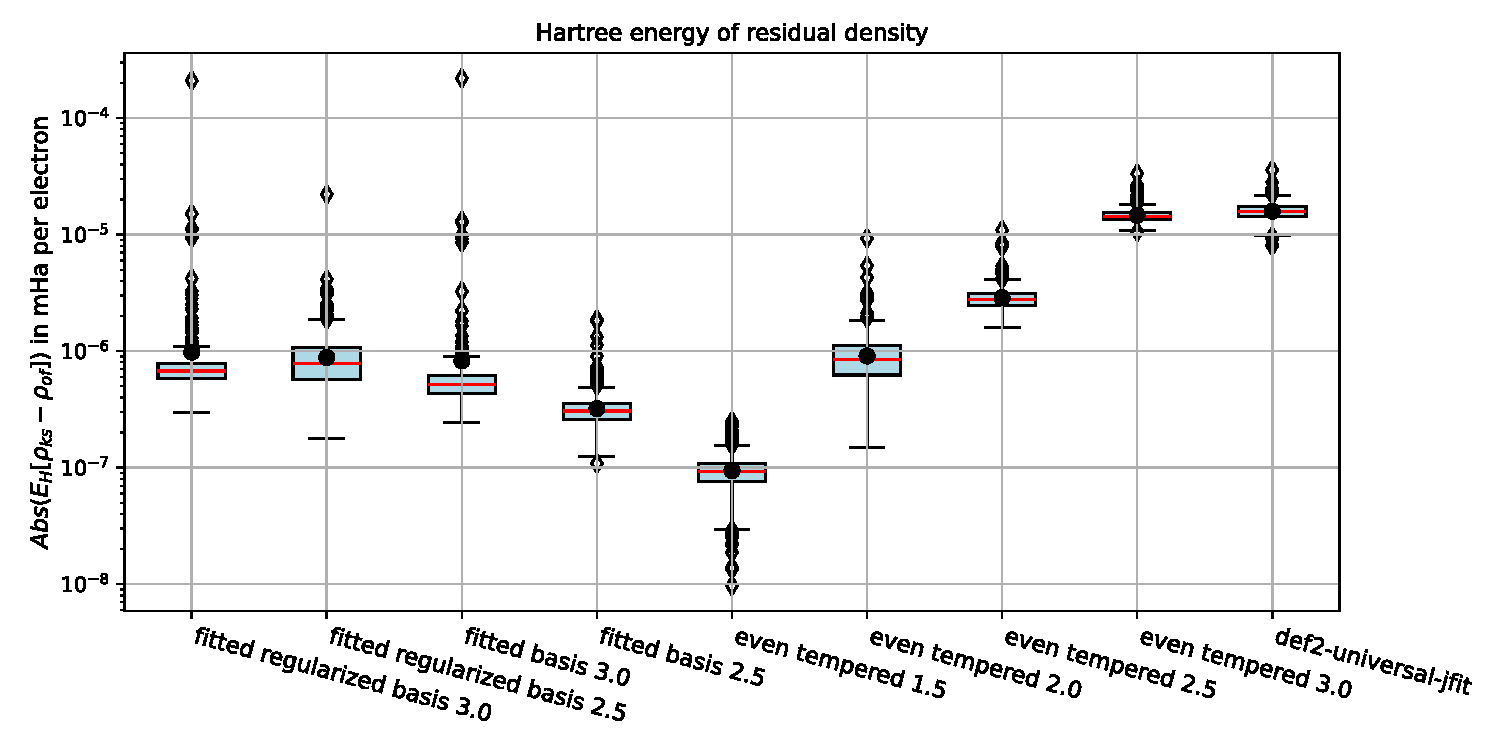
\includegraphics[width=0.6\textwidth]{chapters/results/results_images/L2_residual_hartree_on_hartree+external_MOFDFT_for_different_basis_sets}
    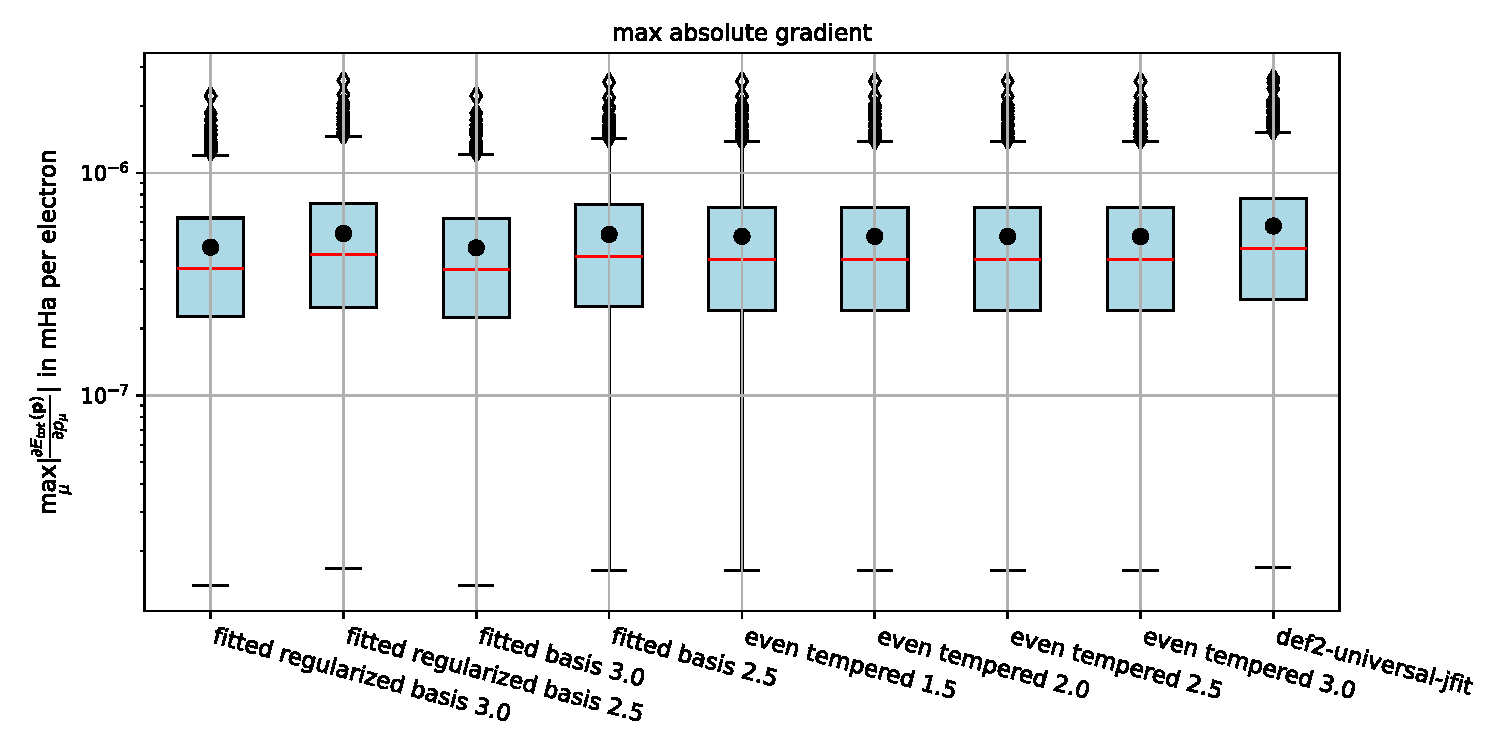
\includegraphics[width=0.6\textwidth]{chapters/results/results_images/max_abs_gradient_on_hartree+external_MOFDFT_for_different_basis_sets}
    \caption{Comparison of the different losses used to fit the basis set}
\end{figure}


 \begin{figure}
   \centering
   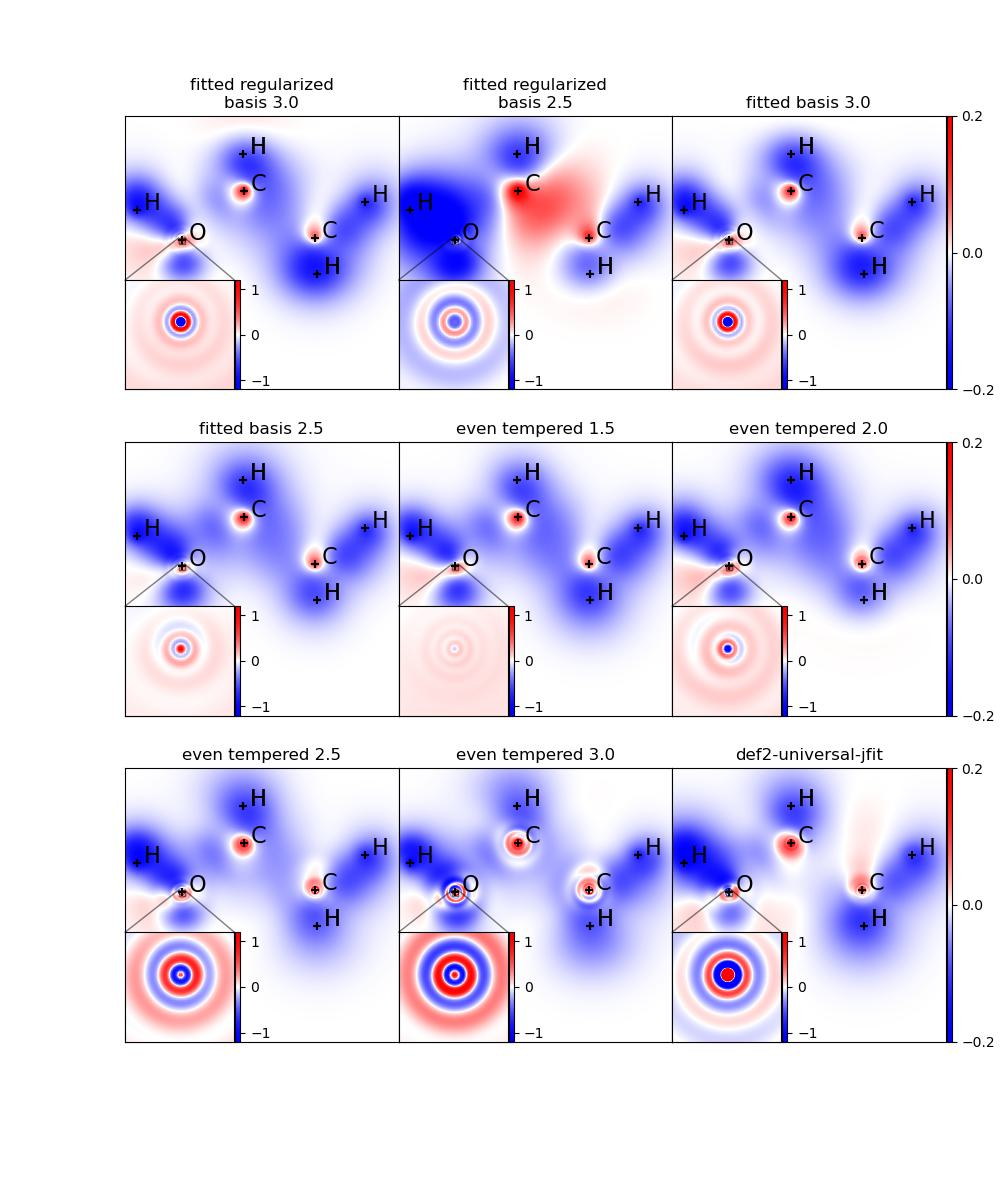
\includegraphics[width=1\textwidth]{chapters/results/results_images/density_fitting_slices2}
     \caption{Slices of the fitted density with density fitting method hartree+external Mofdft using different basis sets}
 \end{figure}

\begin{figure}
    \centering
    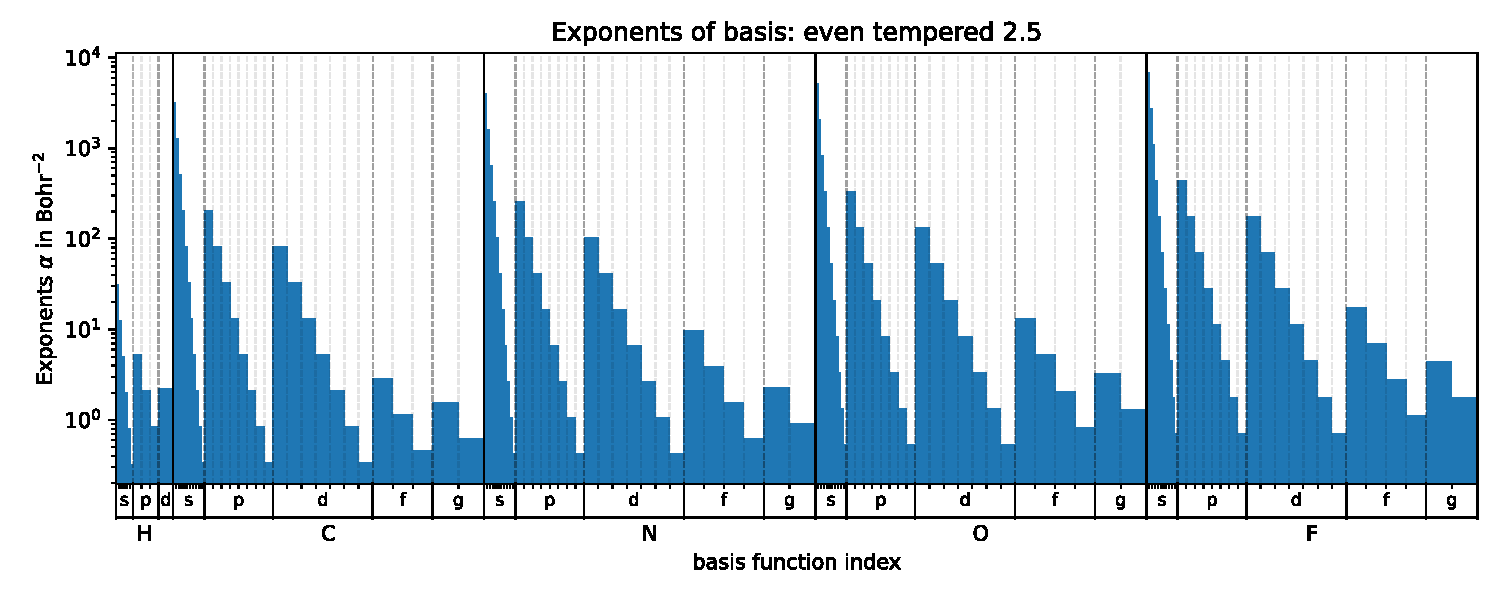
\includegraphics[width=0.6\textwidth]{chapters/results/results_images/basis_functions_even_tempered_2.5}
    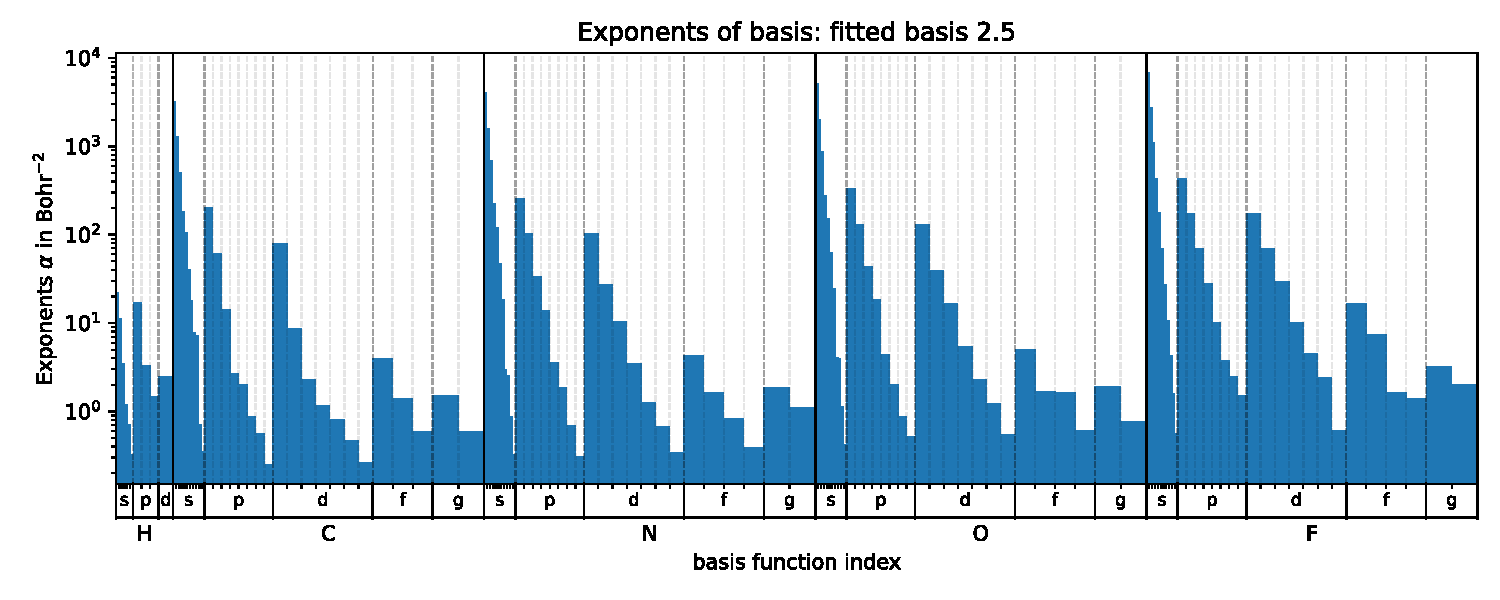
\includegraphics[width=0.6\textwidth]{chapters/results/results_images/basis_functions_fitted_basis_2.5}
    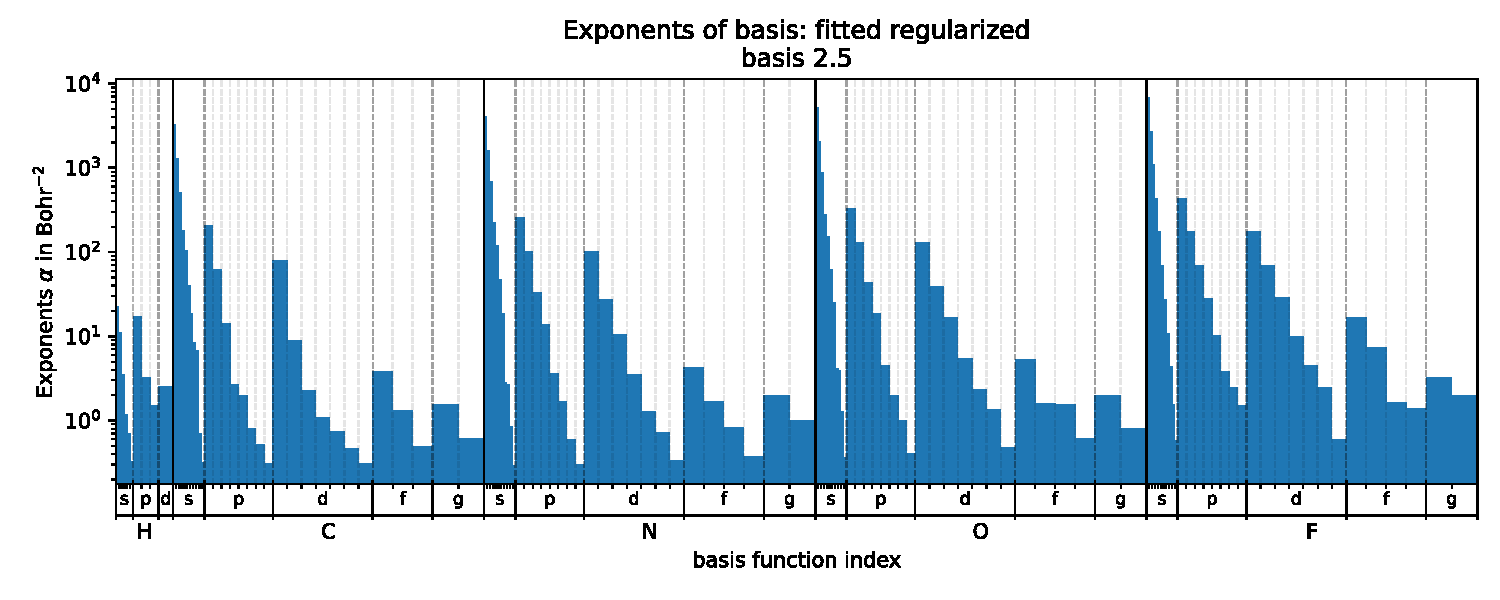
\includegraphics[width=0.6\textwidth]{chapters/results/results_images/basis_functions_fitted_regularized
basis_2.5}
    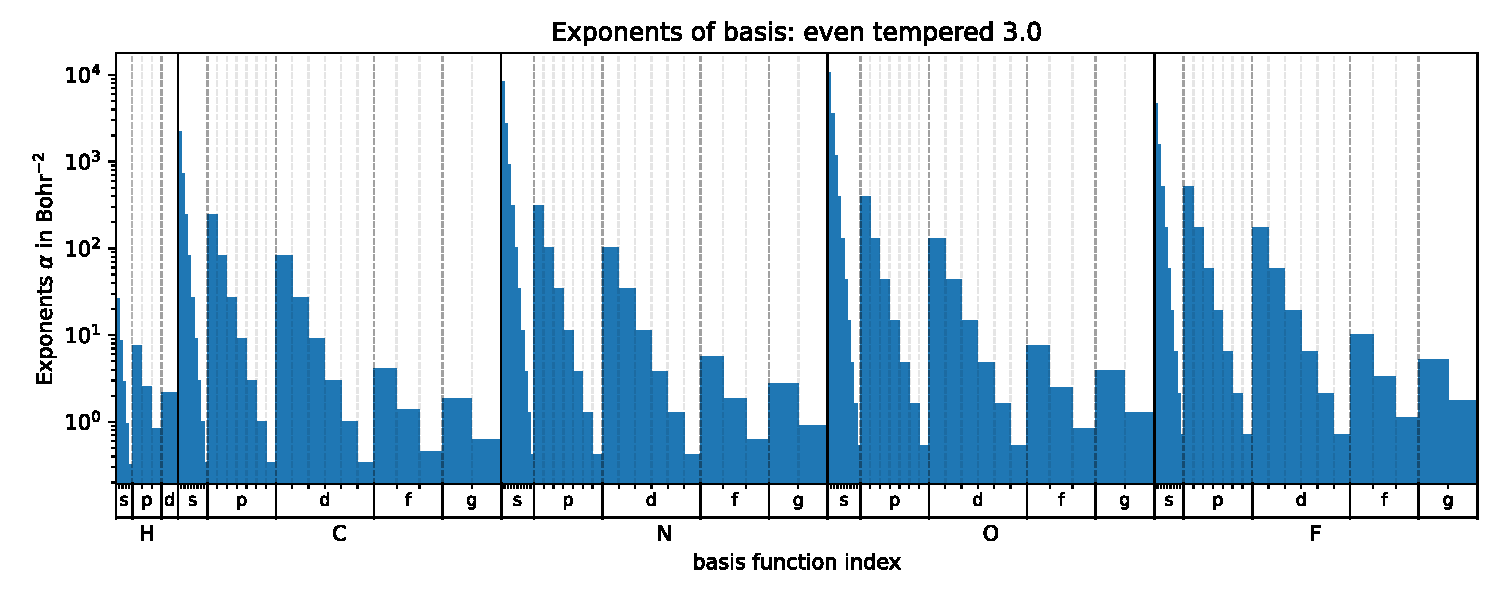
\includegraphics[width=0.6\textwidth]{chapters/results/results_images/basis_functions_even_tempered_3.0}
    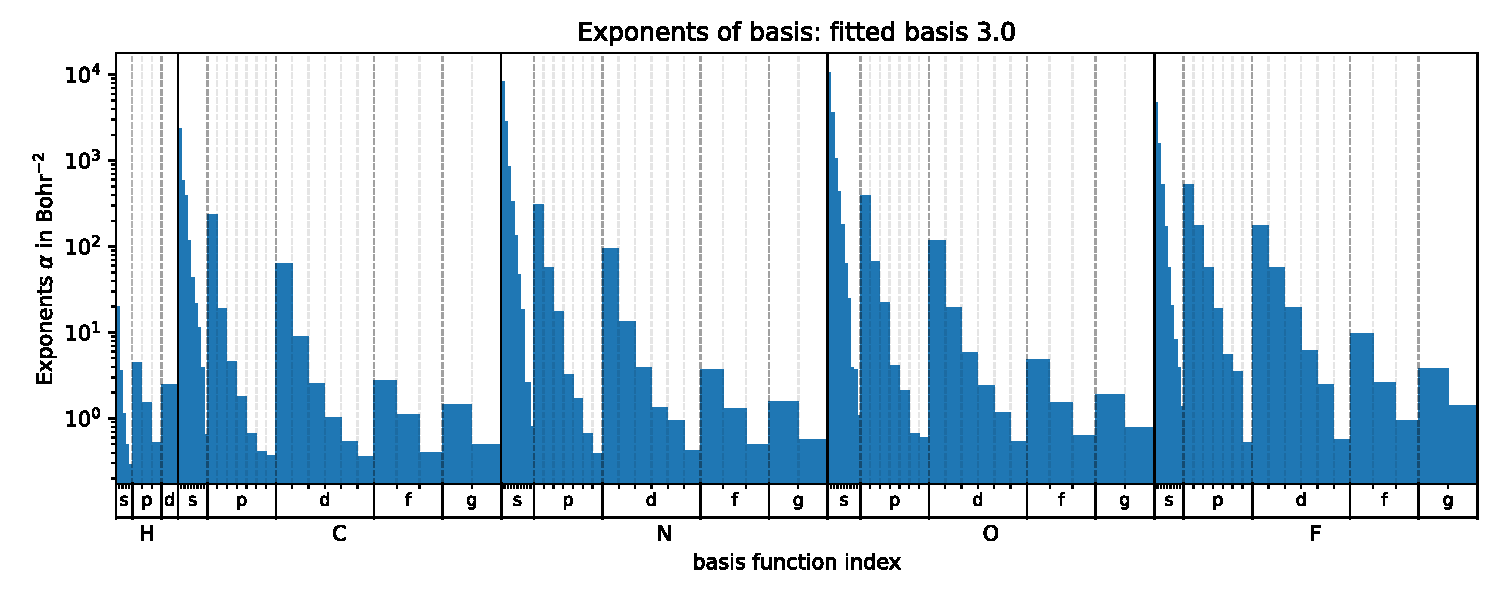
\includegraphics[width=0.6\textwidth]{chapters/results/results_images/basis_functions_fitted_basis_3.0}
    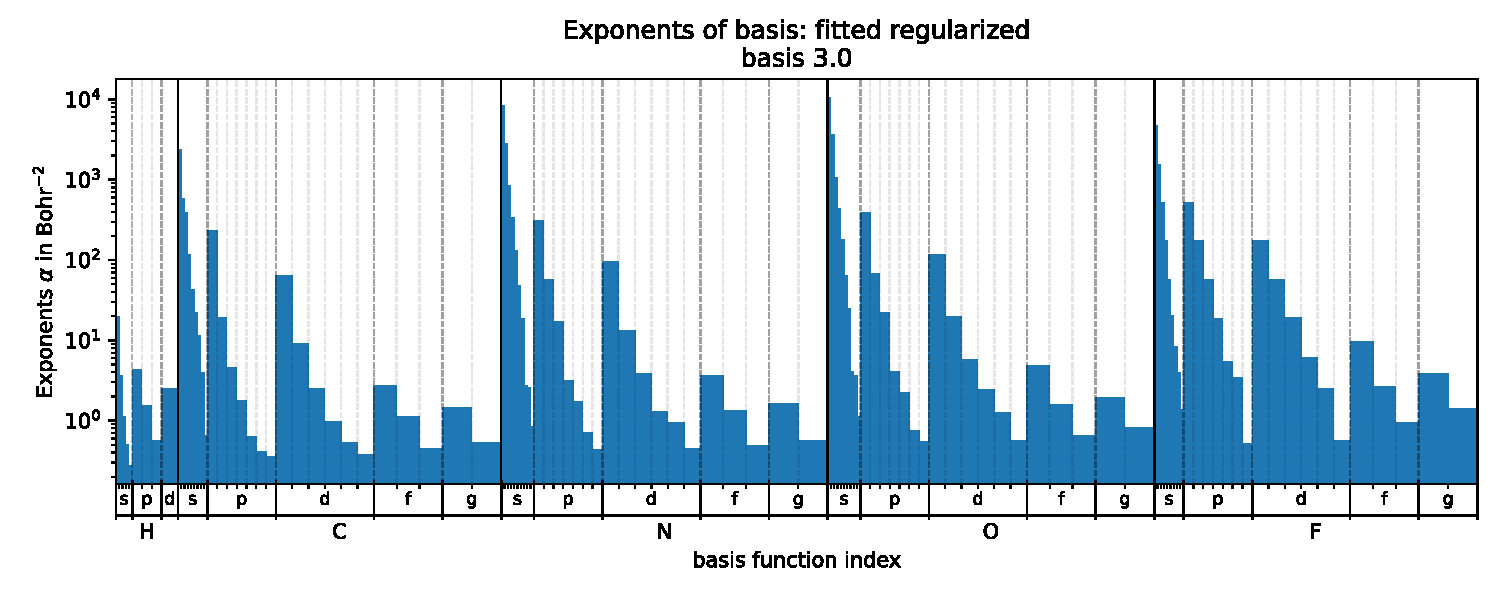
\includegraphics[width=0.6\textwidth]{chapters/results/results_images/basis_functions_fitted_regularized
basis_3.0}
    \caption{Comparison of the different losses used to fit the basis set}
\end{figure}
 







